\chapter{Introduction}

To utilize what we learned in semester 2 and also with the self-accumulated knowledge throughout the semester, we designed this Digital Alarm clock as a fulfilment for the final assignment of the EN1093 module. It is a fully functional and programmable digital alarm clock with Buzzer as sound output.
We are using a DS1307 RTC module with a battery backup power input to store and manage time. We are using $I2C$ protocol to manage the RTC module. Apart from that Atmega 328P will handle all other storage, processing and input/output tasks. $16\times2$ LCD display is used to display time, dates, alarms and other UI components such as menus and tones. A $4\times3$ keypad is used for the user inputs and UI controls. A separate button is added for the alarm interruptions. There is a Factory reset button located inside the enclosure which requires a pin to click it. RTC module, LCD display, Piezo Buzzer, keypad, reset and Stop buttons are directly connected to the Atmega 328P Micro Controller. For reprogramming the microcontroller, there is a serial input reserved in the PCB.


\section{Problem Statement}

Designing a Digital Alarm clock, with all the conventional features and minimalist design to reduce the cost but keeping a good user experience.



\chapter{Method}

\section{Steps of the Project}

Using teamwork and step by step process, we were able to finish this project. These are the main steps we followed

\begin{minipage}{0.97\textwidth}
\centering

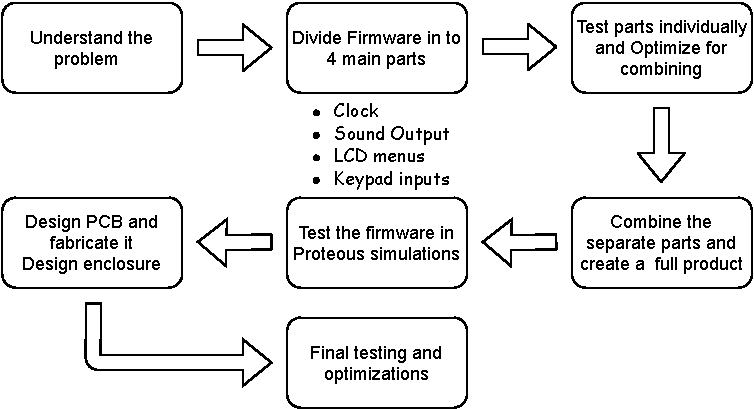
\includegraphics[width=\textwidth]{step.pdf}
\captionof{figure}{Steps}
\end{minipage}

After printing the PCB, the final stage of testings were started. All the components and PCB details is available in the Appendix

\section{COMPONENTS AND THEIR ALGORITHMS}

Here we will look at the main components and how the algorithms and codes work.

\subsection{The RTC Module}

The DS1307 RTC module is working with the I2C protocol with an inbuilt battery chamber so even when the power is not available, The date and time data will be preserved. Using SCL and SDA pins to connect to the microcontroller. The module is temperature dependable so keeping it separated from the main PCB was a solution for the heating. The I2C libraries that we implemented were created by \href{http://jump.to/fleury}{Peter Fleury}. The chip maintains seconds, minutes, hours, day, date, month, and year information. The date at the end of the month is automatically adjusted for months with fewer than 31 days, including corrections for leap year.

\Large \textbf{Features}
\normalsize
\begin{itemize}
  \item 32KHz Crystal oscillator 
  \item 3V CR2032 battery backup
  \item 32 bytes 24C32 EEPROM	
\end{itemize}
\Large \textbf{Algorithm}\\[0.1cm]
\\*
\normalsize{With I2C address 0xD0. The module is taking and stores data in 24-hour format.}
\begin{itemize}
  \item ds1307\_setdate() Function takes year, month, day, day of week, hour, minute and second in decimal form and send the data to RTC module to rewrite current information. 
  \item ds1307\_getdate() Function is used to pull the above information back to the microcontroller.
\end{itemize}

\begin{minipage}{0.97\textwidth}
 \noindent\makebox[\textwidth]{
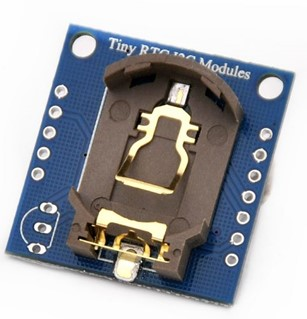
\includegraphics[width=0.5\textwidth]{Picture3.jpg}

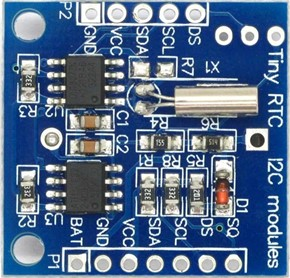
\includegraphics[width=0.45\textwidth, angle=90]{Picture2.jpg}}\hfill
\end{minipage}




\subsection{Buzzer}

The Active piezo buzzer is the Sound output device in the Alarm Clock and it used Square waves to generate tones. The pitches header file contains the keys and their designated frequencies. Using this pitch data, time ratios and provided tempo data given in the melodies header file will be used to generate tone sequences. The negative time ratio sequences indicate extended tones. Positive ones are shorter. There are 5 songs and these will be used to trigger the alarm alerts. This data is stored in Program memory to utilize the storage properly. We will use the PD2 pin to connect The buzzer to Atmega 328P.The melodies are adapted from the works of \href{https://github.com/robsoncouto}{Robson Couto}.


\Large \textbf{Features}
\normalsize
\begin{itemize}
  \item Active Buzzer 
  \item Using amplifier for better sound volume created with a BJT
  \item The diode across the buzzer prevent sudden voltage spikes and protect the BJT	
\end{itemize}
\Large \textbf{Algorithm}\\[0.1cm]
\\*
\normalsize{To generate a tone out of the buzzer, it needs a signal with that specific frequency. Using simple delays and toggling the output pin we can archive this while generating 50\% duty cycle square waves. Since this part is also working as the Alarm output, to implement an interrupt to the system we will use external interrupt pin PD3 to utilize this. Upon the rising edge high, the tone playing function will stop.}
\begin{itemize}
  \item Play\_Note() Function is used to generate 50\% duty square waves when the relevant frequency and the time duration is given.  First, generate the time duration per cycle and then calculate the number of cycles. For each cycle turn 50\% of time output high and then turn output low for the remaining 50\% cycle. Repeat this for all cycles. If the input frequency was 0, then the output will be 0 for the given duration. 
  \item Play() function will take single integer input which is the song number. After that reading values from the melodies header, it will take notes and duration and trigger Play\_Note() function with the predetermined length and tempo will be used to generate the tone duration. The external interrupt button can be used to stop this function and stop the sound from playing.
\end{itemize}


\begin{minipage}{0.97\textwidth}
 \noindent\makebox[\textwidth]{
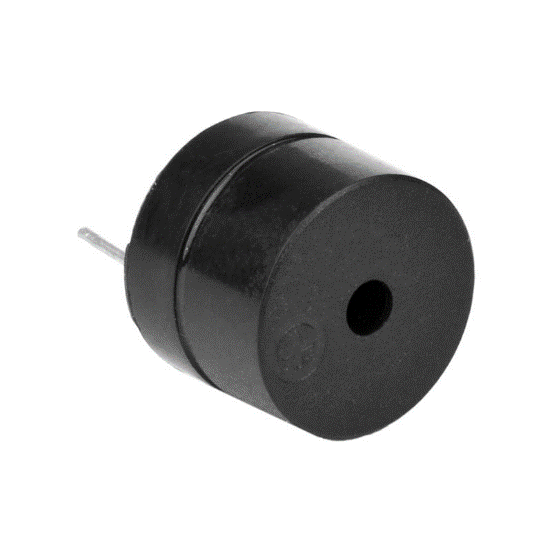
\includegraphics[width=0.5\textwidth]{Picture4.png}
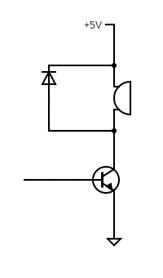
\includegraphics[width=0.3\textwidth]{Picture5.png}}\hfill
\end{minipage}



\subsection{LCD Display}

This 16-character, 2-line parallel liquid crystal display achieves a large viewing area in a compact package. The DDRAM address 0x00 corresponds to the first character of the top line, address 0x0F corresponds to the last character of the top line, address 0x40 corresponds to the first character of the second line, and address 0x4F corresponds to the last character of the second line.

The main functionality of the LCD is to display
\begin{itemize}
  \item Time/Date 
  \item Control menus
  \item Tone selections	
\end{itemize}
We are utilizing maximum contrast by grounding the $V_{0}$,$V_{EE}$ pin and 4bit configuration mode. Total 6 pins are connected with the microcontroller using a male-female connector. The datasheet will be provided.

\Large \textbf{Features}
\normalsize
\begin{itemize}
  \item Using 4Bit mode to utilize pins efficiently  
  \item Blue backlight
  \item Looks Stylish	
  \item Always-on display	
\end{itemize}
\vspace{0.2cm}
\Large \textbf{Algorithm}

\normalsize{All the menus and content displaying will be done by this algorithm.}
\begin{itemize}

  \item displayTime() will be used to display the time and date on the main screen. The data for this display option will be taken from the RTC module.. 
  \item LCD\_SetAlarm() Function is used to take user inputs from the 4x4 keypad and set one alarm at a time. To reach this point user will have to choose from “Set Alarm” from the listed menu.
  \item LCD\_Tone() Function will display currently available Alarm tones. The alarm tone names are stored In an array named tone\_List. You can select a tone and this function will give an integer output for the selected song index.
  \item LCD\_SetDate() This function will grant the user to update system tie and date with the help of keypad inputs.
\end{itemize}
\vspace{10mm}
\centerline{
\begin{minipage}[t]{0.8\textwidth}

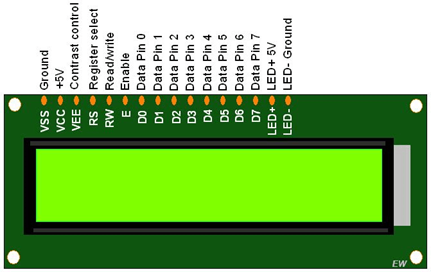
\includegraphics[width=\textwidth]{Picture6.png}

\end{minipage}}

\newpage
\subsection{Keypad input}

We are utilizing a $4\times3$ matrix keypad for our input purposes. Using number keys as basic number inputs as well as for menu navigation

\normalsize
\begin{itemize}
    \item 8 :- UP
	\item 2 :- DOWN
	\item \#:-RETURN/ CANCEL
	\item * :- ENTER/ SELECT
\end{itemize}

\Large \textbf{Features}
\normalsize
\begin{itemize}
  \item Active Buzzer 
  \item Using amplifier for better sound volume created with a BJT
  \item The diode across the buzzer prevent sudden voltage spikes and protect the BJT	
\end{itemize}

use 7 pins for communication with the Microcontroller.
\vspace{5mm}

\Large \textbf{Algorithm}

\normalsize{In a nutshell, keypad works as a matrix of push buttons. There are 4 output pins (PC0 to PC3), and the inputs will be toggled in a sequence from top raw to bottom raw. In a instance if a button is pressed we can recognize that row with the toggled on pin. At instance of the button is pressed, that input pin will toggle 5V accordingly. There are 3 input pins (PB0 to PB2). They are connected using a pull down resistor. By the column and raw number, system can recognize the pressed button.}

\begin{itemize}
  \item btnPress() function will check the pins and ports and return the character given in the location reading the matrix data. We will utilize this to get properly control the inputs. 
\end{itemize}



\begin{minipage}{0.97\textwidth}
 \noindent\makebox[\textwidth]{
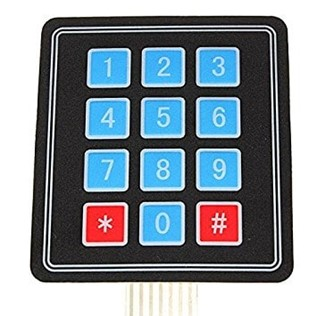
\includegraphics[width=0.5\textwidth]{Picture7.jpg}
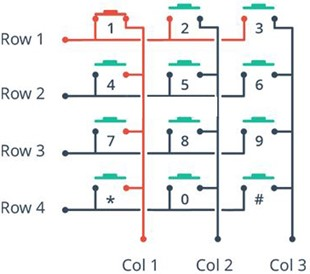
\includegraphics[width=0.5\textwidth]{Picture8.jpg}}\hfill
\end{minipage}

\newpage
\section{Features and Overall working Methodology}
Here we will look at the features and how the overall algorithm work.
\vspace{5mm}
\subsection{Displaying Time and date}

After startup and after the Welcome screen, the date and time data will be constantly be pulling out of the RTC module. And with the LCD display, it will keep updating accordingly. This process doesn’t have any specified delays. It will constantly do this process till a key input is given.

\begin{center}
  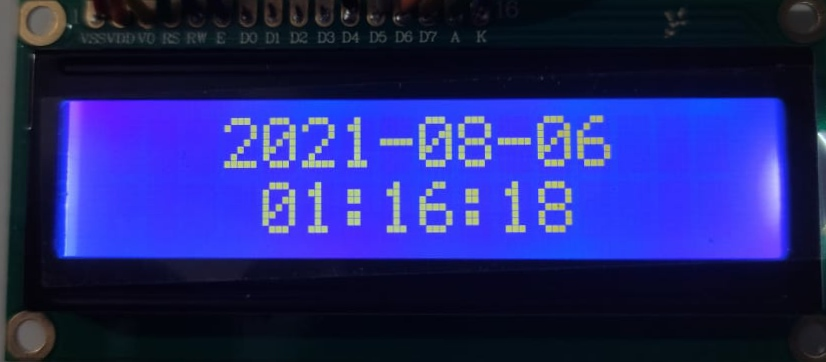
\includegraphics[width=8.5cm]{LCD Images/LCD 1.jpg}
  \captionof{figure}{Time and date}
\end{center}

After a key input, It will navigate to the First list containing
\begin{enumerate}
\item SET ALARM
\item SET TIME
\item SEE ALARMS
\item TIMER
\end{enumerate}
%\vpace{}
\subsection{Selecting sub menus and features.}
Here we will check each scenario.

\subsubsection{SET ALARM} 
If you select $SET \: ALARM$, it will navigate to a new screen where you need to enter the alarm details and you can use the keypad numbers to enter the alarm time. The Alarm should be inserted in hh:mm order. After that pressing “ $* $“  will take to the next stage to select an alarm tone. To navigate the list up and down, the 2 and 8 buttons are reserved. After choosing the alarm, alarm is set. The algorithm will update a list of arrays with the Alarm Time and Chosen Tone data. These data will be linked by an index.

\begin{minipage}{0.97\textwidth}
 \noindent\makebox[\textwidth]{
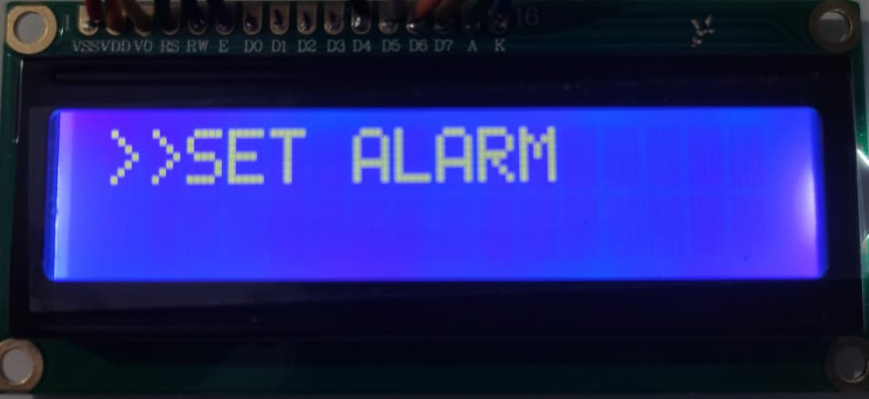
\includegraphics[width=0.5\textwidth]{LCD Images/LCD 2.jpg}
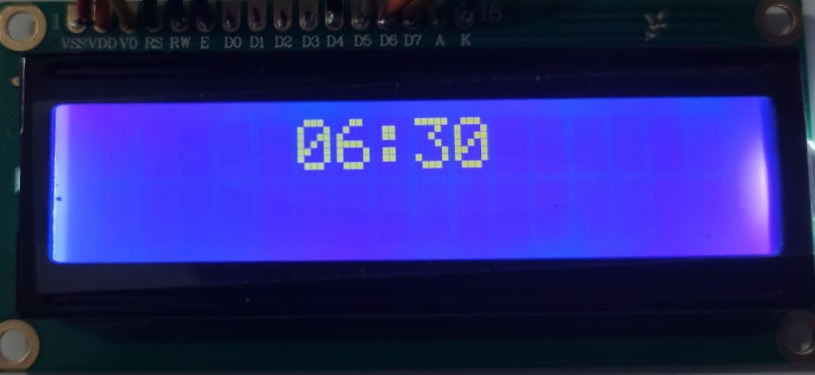
\includegraphics[width=0.5\textwidth]{LCD Images/LCD 3.jpg}}\hfill
\noindent\makebox[\textwidth]{
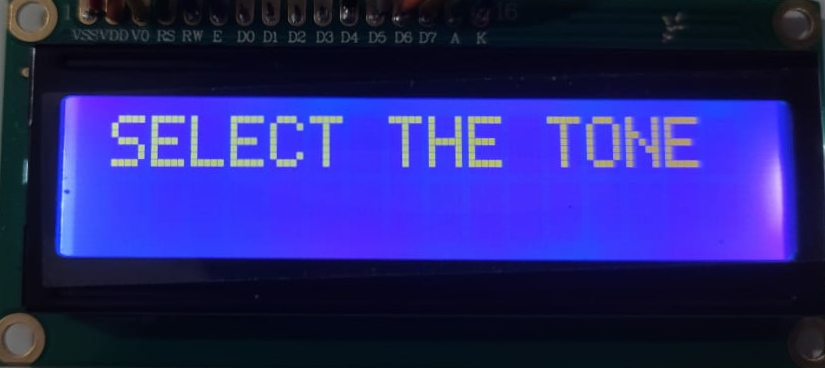
\includegraphics[width=0.5\textwidth]{LCD Images/LCD 4.jpg}
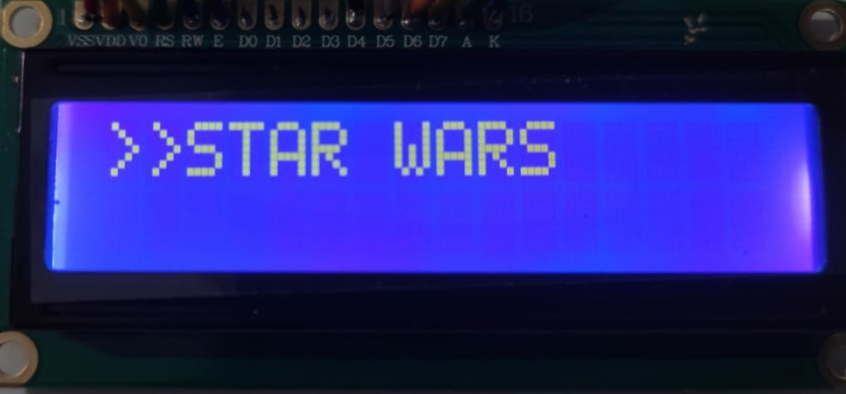
\includegraphics[width=0.5\textwidth]{LCD Images/LCD 5.jpg}}\hfill
\captionof{figure}{Setting An Alarm LCD Menus}
\end{minipage}



\subsubsection{SET TIME} 
If you select $SET\:TIME$, it will open a new screen to set alarm and time. Using keypad inputs date should be added in $yyyy/mm/dd$ format and time in $hh:mm:ss$ format. After setting time this data will be sent to RTC module with the ds1307\_setdate() function.

\begin{center}
  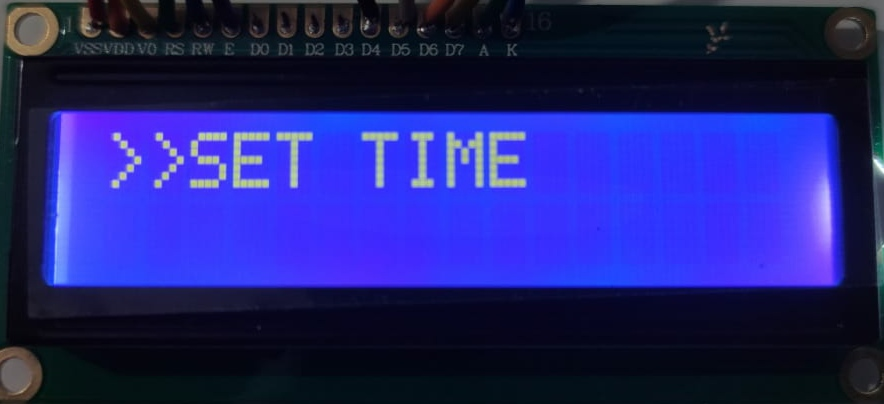
\includegraphics[width=8.5cm]{LCD Images/LCD 6.jpg}
  
  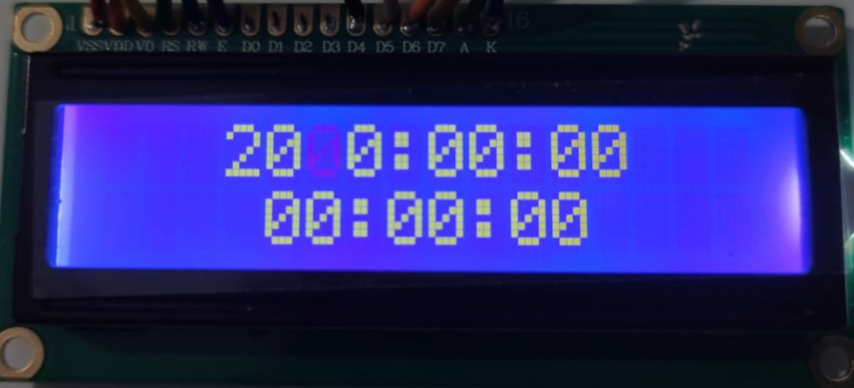
\includegraphics[width=8.5cm]{LCD Images/LCD 7.jpg}
  \captionof{figure}{Changing LCD Menus}
\end{center}
\newpage
\subsubsection{SEE ALARMS} 
If you select $SEE \: ALARMS$, you can see all the currently available Alarms. If there is Non, A No alarms message will be displayed. From here you can delete alarms as you please. “5” Key is reserved for that purpose. User can remove any and all alarms, if the list is empty, it will say that.


\begin{minipage}{0.97\textwidth}
 \noindent\makebox[\textwidth]{
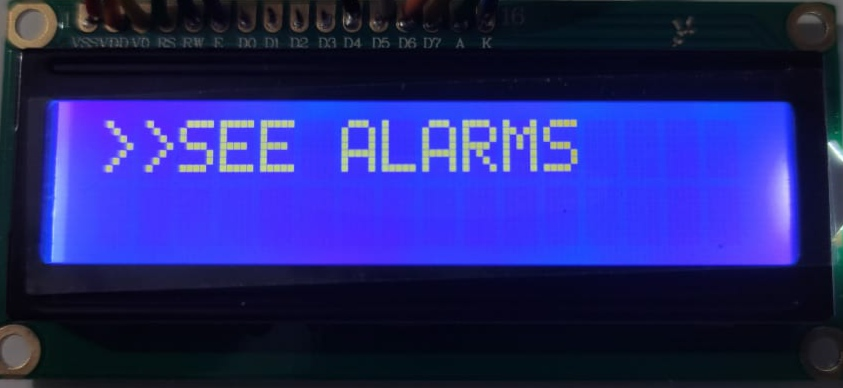
\includegraphics[width=0.5\textwidth]{LCD Images/LCD 8.jpg}
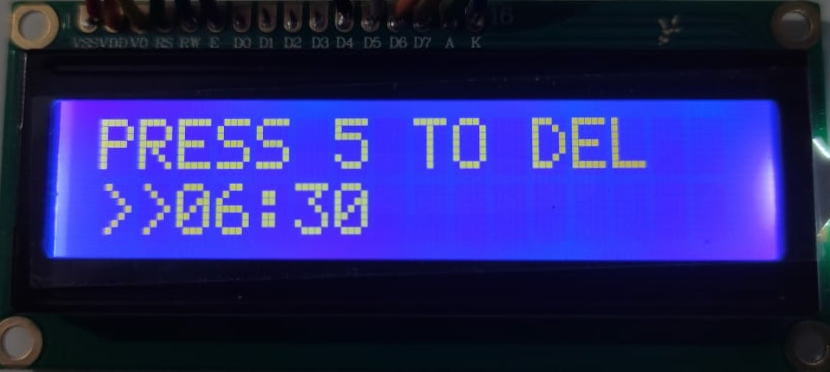
\includegraphics[width=0.5\textwidth]{LCD Images/LCD 9.jpg}}\hfill
\noindent\makebox[\textwidth]{
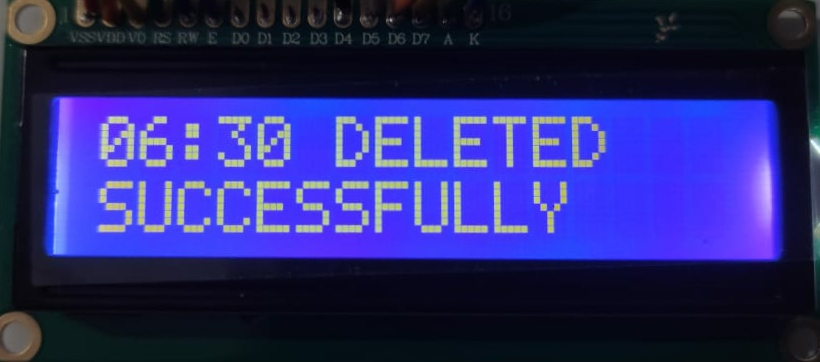
\includegraphics[width=0.5\textwidth]{LCD Images/LCD 10.jpg}
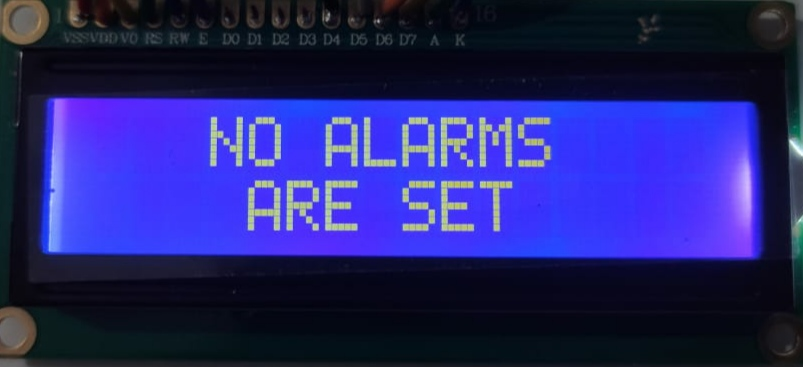
\includegraphics[width=0.5\textwidth]{LCD Images/LCD 11.jpg}}\hfill
\captionof{figure}{Available Alarm list LCD Menus}
\end{minipage}


\subsubsection{TIMER}

$TIMER$ will give you a countdown timer. You can set how long of a timer you need by setting the time in $hh:mm:ss$ format. After the timer reach 00:00:00, Star Wars Imperial march theme will be played.

\begin{minipage}{0.97\textwidth}
\centering
\makebox[\textwidth]{
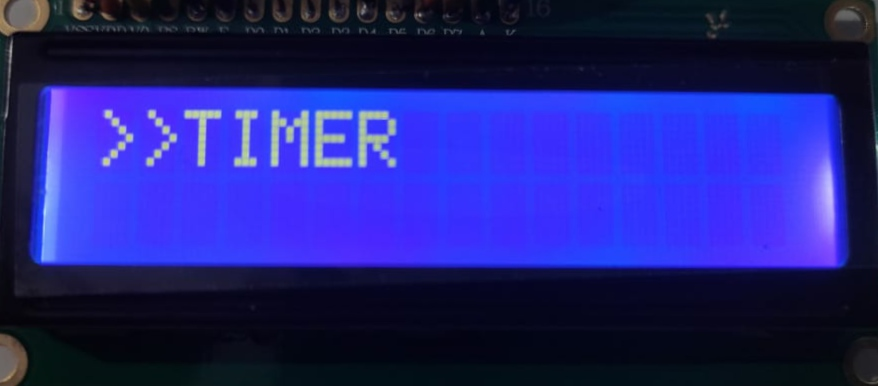
\includegraphics[width=0.5\textwidth]{LCD Images/LCD 12.jpg}
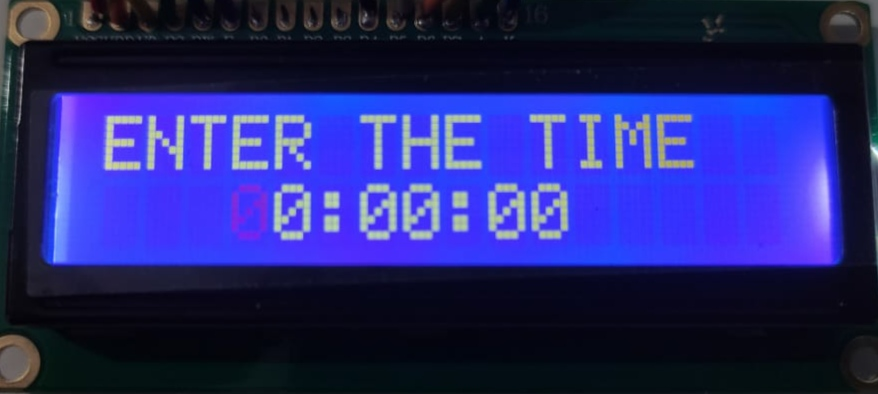
\includegraphics[width=0.5\textwidth]{LCD Images/LCD 13.jpg}}\hfill
\centering\makebox[\textwidth]{
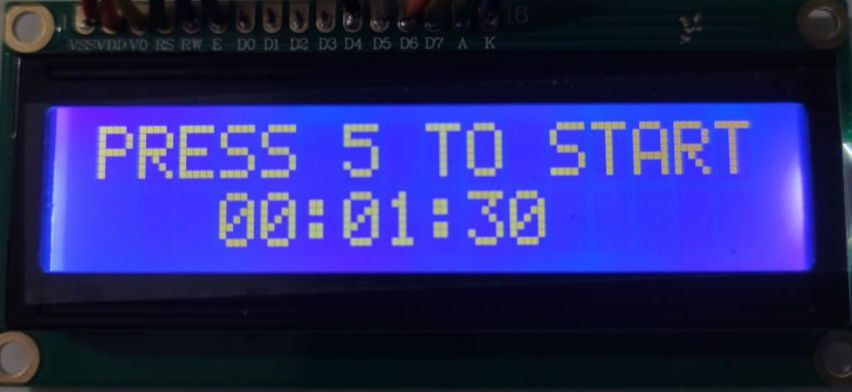
\includegraphics[width=0.5\textwidth]{LCD Images/LCD 14.jpg}
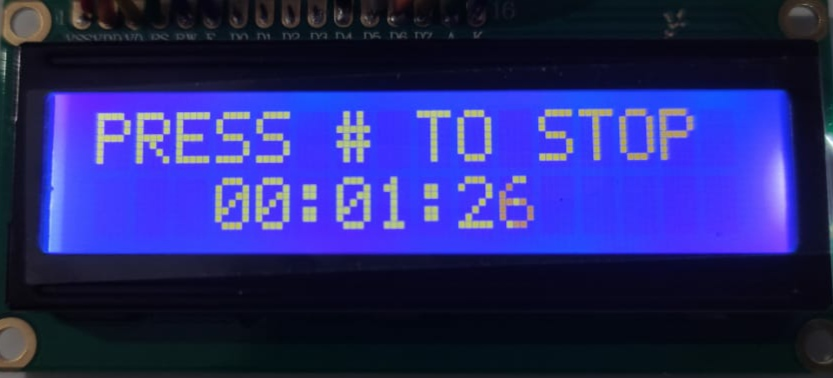
\includegraphics[width=0.5\textwidth]{LCD Images/LCD 15.jpg}}\hfill
\captionof{figure}{Timer LCD Menus}
\end{minipage}
\newpage
\subsection{Alarm interrupting}
Since Alarms usually get abused when stopping alarm, we added a separate, durable and big button for this purpose. By using external interrupt pins, the “$sp$” variable will be changed to 0. Using this even when the microcontroller is busy with the for loop, checking this variable can be used to stop the buzzer music from playing.
\subsection{Factory resetting}
Using the inbuilt reset pin, which is also shared with the programmer, the factory resetting
Will be done. The push button will reset everything except the RTC module because it has a separate memory inside. In the enclosure a pin cutout is provided for the user to push the hidden button with a pin. This will stop accidental button presses.

\subsection{Programmer}

Since our goal was to create a re-programmable digital alarm clock, there is an inbuilt programmer pin reserved header. Using either a USB to serial/TTL programmer or an Arduino device, user can flash firmware. The source code is available in \href{https://github.com/dakshinatharindu/Digital-Alarm-Clock}{this} GitHub Repository.

\chapter{Results}
Our PCB design was working as intended but one pin in LCD header was not grounded. The Buzzer had a good volume. The LCD had a contrast issue but was able to fix it by placing a resistor in the pin 3. The current usage was good. The keypad had good responses, the debouncing effect was in an acceptable range. After continuous run over a week, the Time in the RTC module was not affected.

\begin{minipage}{0.97\textwidth}
 \noindent\makebox[\textwidth]{
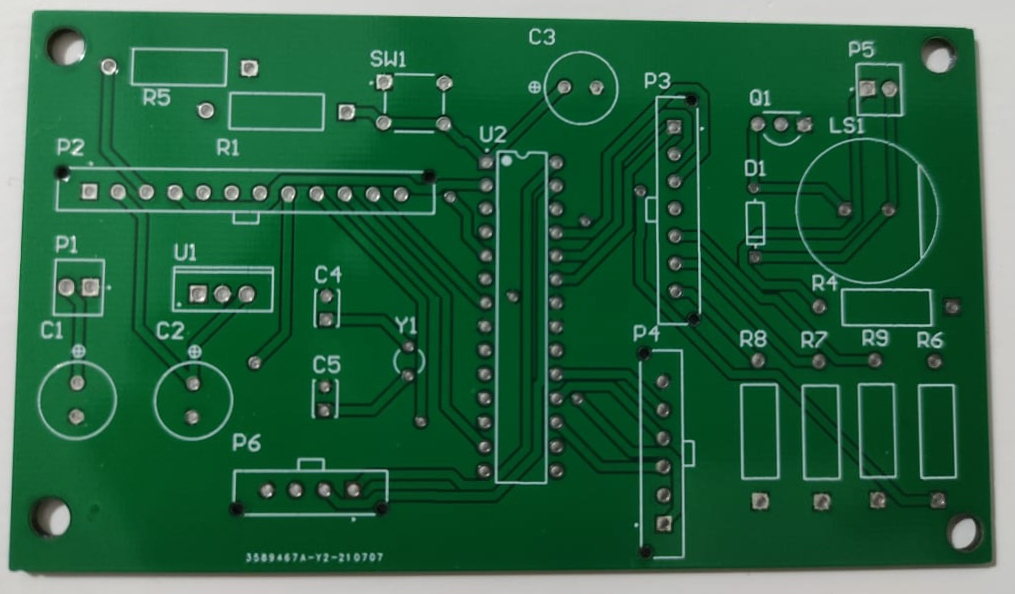
\includegraphics[width=0.5\textwidth]{PCB fabricated/PCB no-solder top.jpg}
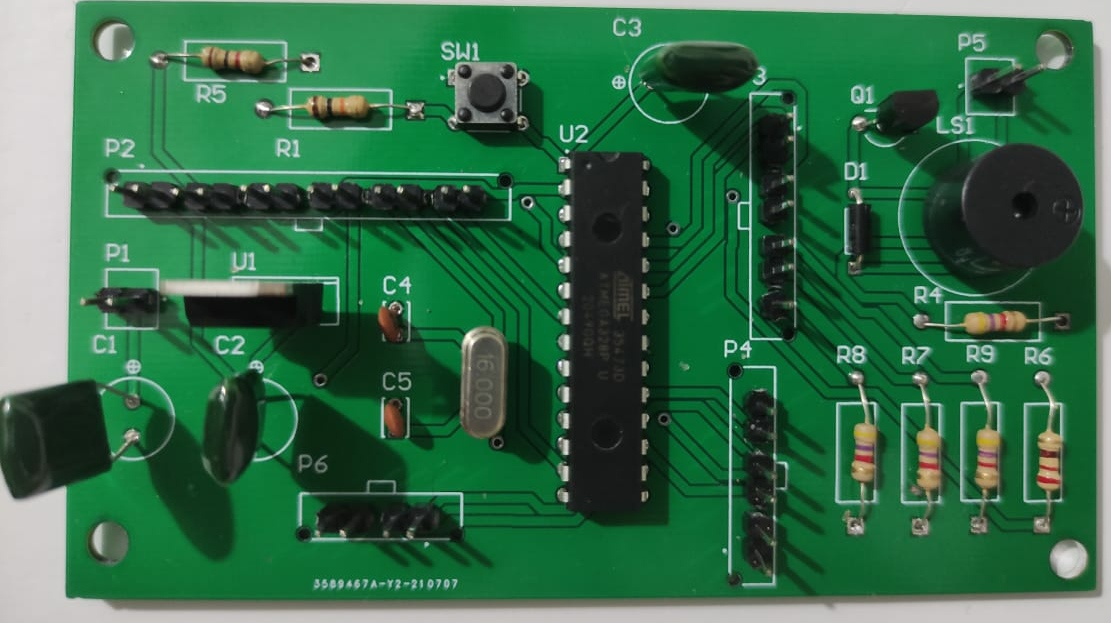
\includegraphics[width=0.5\textwidth]{PCB fabricated/PCB solder top.jpg}}\hfill
\noindent\makebox[\textwidth]{
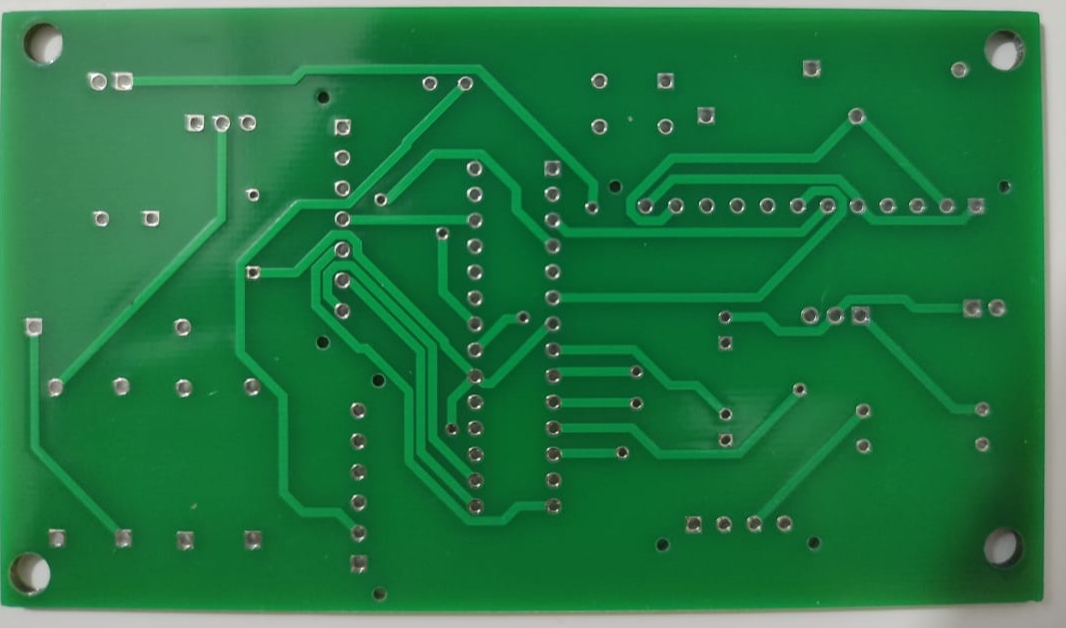
\includegraphics[width=0.5\textwidth]{PCB fabricated/PCB no-solder bottom.jpg}
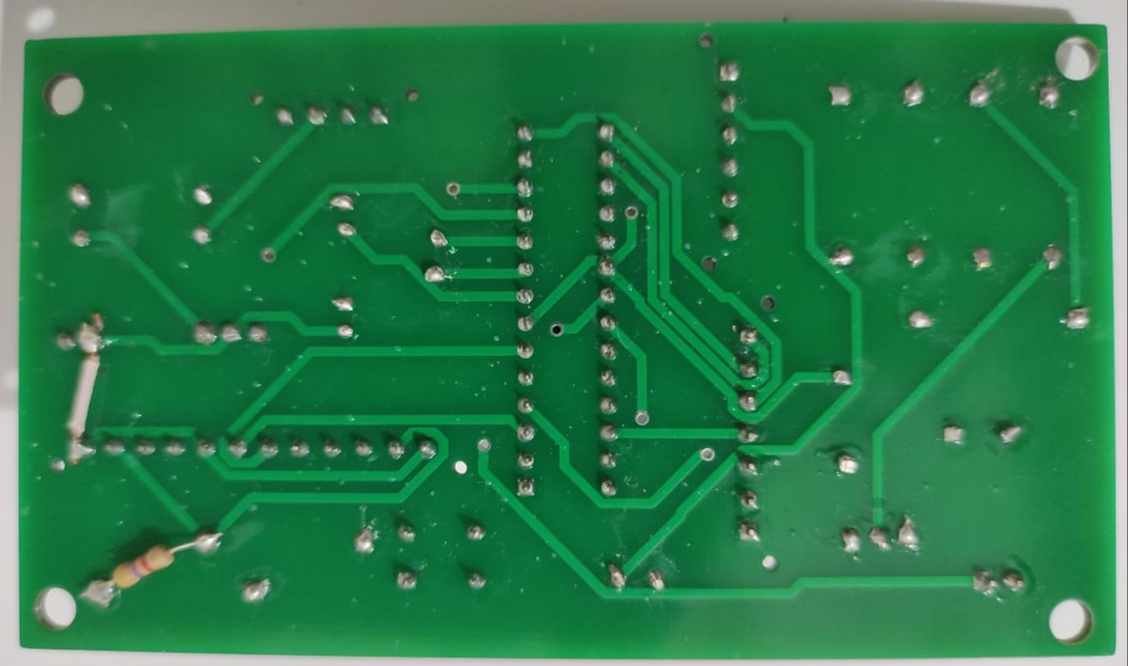
\includegraphics[width=0.5\textwidth]{PCB fabricated/PCB solder bottom.jpg}}\hfill

\end{minipage}

As for our enclosure design, we were not able to 3D print it due to quarantine and other issues.\\
\begin{minipage}{0.97\textwidth}
 \noindent\makebox[\textwidth]{
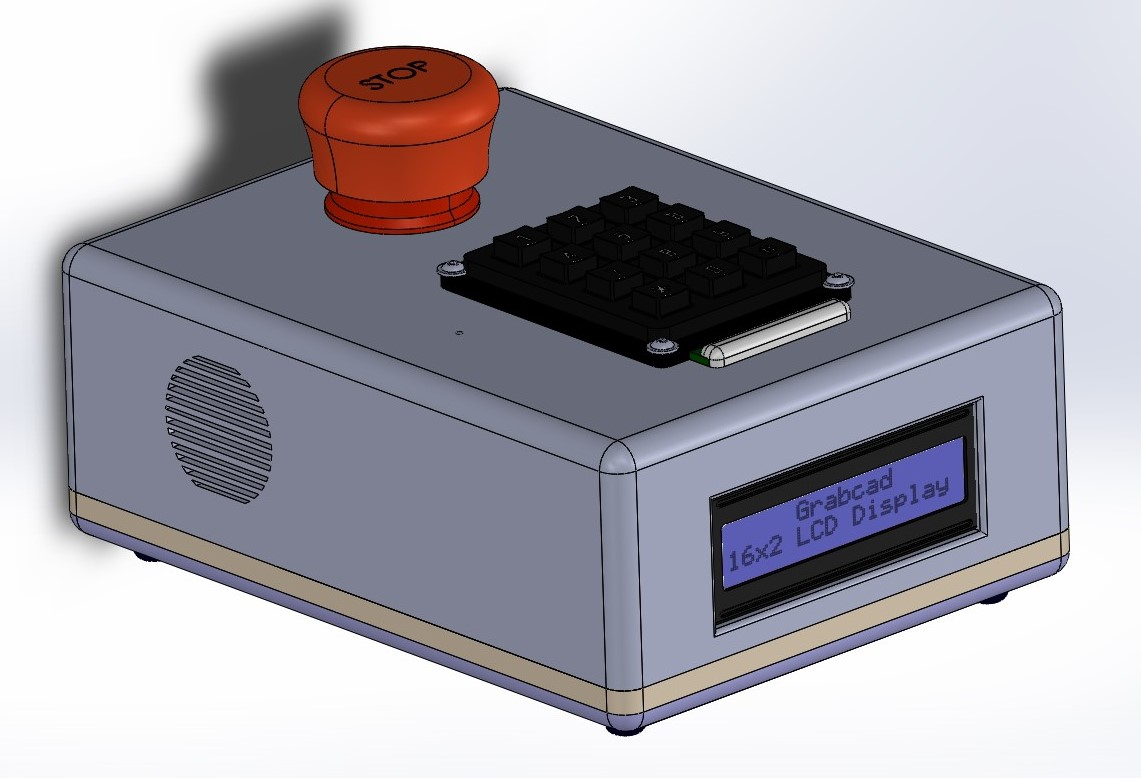
\includegraphics[width=0.5\textwidth]{Enclosure/Solid.jpg}
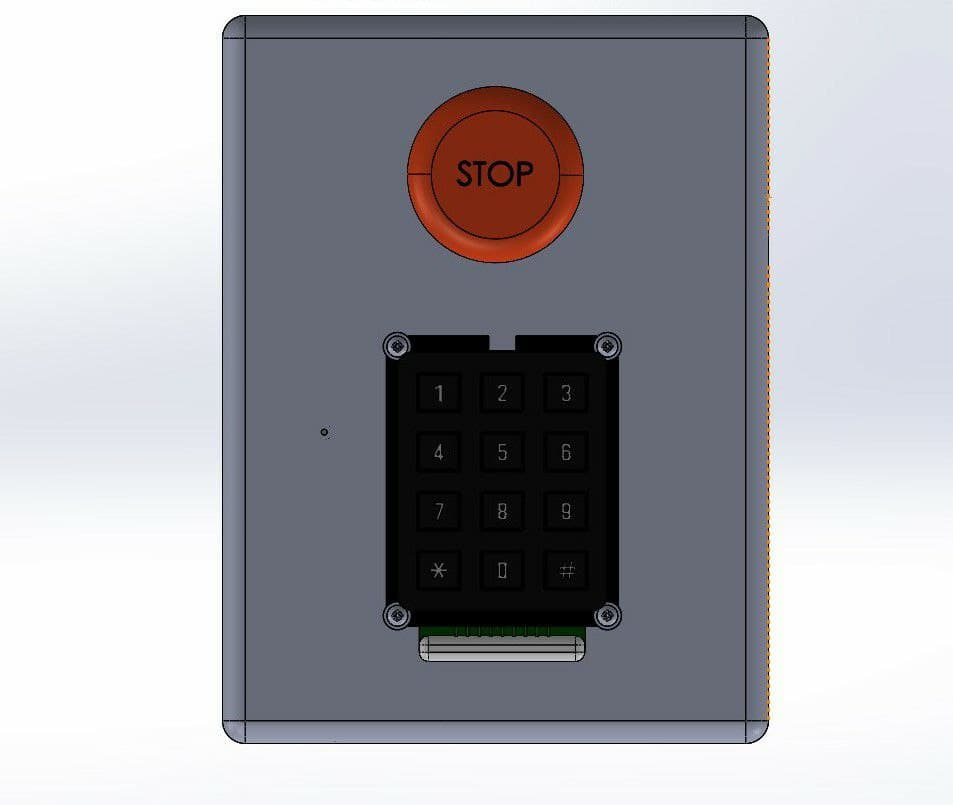
\includegraphics[width=0.5\textwidth]{Enclosure/solid2.jpg}}\hfill
\end{minipage}
\newpage
\chapter{Discussion}
As beginners for the embedded designing, we had to learn all the software such as,
\begin{itemize}

\item Proteus
\item Altium designer
\item Solidworks 

\end{itemize}

from the fundamentals.\\
Also, this was the first time we were introduced to AVR C++ and, we did not have much background in C language.We had to learn AVR C++ from the basics.

\section{Problems and challenges we faced during this project}

\begin{itemize}
\item Since the start of the semester, due to COVID 19 pandemic, our team was not able to collaborate in person.
\item We had problems with acquiring few parts we needed for our product.
\item The deliveries were delayed. So we had to wait for the ordered parts to come for a long time.
\item Due to a manufacturing error, our PCB had an unrouted pin.
\item Proteus simulations have frequency issues. So we had to alter codes many times for the buzzer. Due to this problem we are using $1MHz$ internal frequency.
\item LCD display had too high a contrast level, we had to connect a resistor in order to get proper readability.
    
\end{itemize}

\section{Overall impression and possible improvements}
Even though we were not able to 3D print our enclosure design and test it, our design has a good durability and the practicality. The basic box design is suitable for keeping internal components safe from hard impacts. The external button for stopping the alarm is really useful when the user is in a hurry and if the impact is high.The buzzer volume is load and the alarm tones are in a wide range of styles for user to choose.

Since there is no mechanism to change the LCD brightness level, this might become a problem for some scenarios. We will fix this issue and add a option to change screen timeout time.
\newpage
Overall, the project was a tremendous success, both in its operations and in the lessons obtained from taking on such an involved project. It was a really good experience and gave us the push we needed to start our own projects on embedded systems.
We had issues when printing the PCB and finally decided to order the PCB from JLC-PCB. Since from the beginning, when we were writing firmware for our micro products, the codes we wrote were easily combinable and was able to communicate with each parts easily. 

There are few features we would like to add to this design. Adding a snooze option could improve user experience. This can be implemented by using the same interrupt button. We can add a option for this by providing a new settings menu too. Giving access to our 9V battery without removing the whole case is also a good feature to adept.


{\let\clearpage\relax \chapter{Acknowledgement}

}
First of all, we would like to pay our gratitude toward our supervisor/instructor/evaluator Mr. Randima Senanayaka for his guidance and encouragement to overcome this challenge through self study and teamwork. Also, without ENTC family this project would not reach success. We would like to thank all the staff members who helped us throughout this project and semester 2. Our sincere gratitude for all the parties behind providing us with free Solidworks and Altium licenses.\\
The help, encouragement, tutorials we received from all the guest lecturers from $EN1070$ module is invaluable and we would like to pay our gratitude.
